\documentclass[svgnames,11pt]{beamer}
\input{/home/tof/Documents/Cozy/latex-include/preambule_commun.tex}
\input{/home/tof/Documents/Cozy/latex-include/preambule_beamer.tex}
%\usepackage{pgfpages} \setbeameroption{show notes on second screen=left}
\author[]{Christophe Viroulaud}
\title{Tris}
\date{\framebox{\textbf{Algo 04}}}
%\logo{}
\institute{Première - NSI}

\begin{document}
\begin{frame}
    \titlepage
\end{frame}
\begin{frame}
    \frametitle{}

    \begin{center}
        \centering
        \includegraphics[width=8cm]{ressources/cartes.jpg}
        \captionof{figure}{Trier un jeu de cartes est un problème informatique.}
        \label{IMG}
    \end{center}

\end{frame}
\begin{frame}
    \frametitle{}

    \begin{framed}
        \centering Déterminer plusieurs méthodes de tris de données.
    \end{framed}

\end{frame}
\section{Algorithmes de tris}
\subsection{Recherche}
\begin{frame}
    \frametitle{Algorithmes de tris - Recherche}
    \begin{center}
        \centering
        \includegraphics[width=10cm]{ressources/jeu-coeur-melange.png}
        \end{center}
    \begin{activite}
        \begin{enumerate}
            \item Prendre le paquet de cartes mélangées et les étaler sur la table.
            \item Trier les cartes.
            \item Formaliser la méthode utilisée sous forme d'un algorithme.
        \end{enumerate}
    \end{activite}

\end{frame}
\subsection{Tri par sélection}
\begin{frame}
    \frametitle{Tri par sélection}

    \begin{itemize}
        \item Pour chaque carte du tas:
              \begin{itemize}
                  \item Trouver la plus petite carte dans la partie non triée.
                  \item Échanger cette carte avec la première de la partie non triée.
              \end{itemize}

    \end{itemize}

\end{frame}
\begin{frame}

    \begin{center}
        \centering
        \includegraphics[width=10cm]{ressources/jeu-coeur-melange.png}
        \end{center}
        \begin{center}
            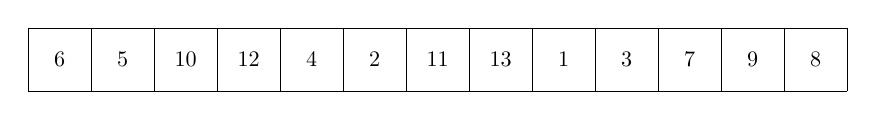
\begin{tikzpicture}[scale=0.8,transform shape]
                \draw (0,0) grid (13,1);
                \foreach \n/\x in {6/0,5/1,10/2,12/3,4/4,2/5,11/6,13/7,1/8,3/9,7/10,9/11,8/12}{
                    \node (\n) at (0.5+\x,0.5) {\n};

                }    
            \end{tikzpicture}
            \captionof{figure}{Modélisation}
        \end{center}

\end{frame}
\begin{frame}


        \begin{center}
            \begin{tikzpicture}[scale=0.8,transform shape]
                \draw (0,0) grid (13,1);
                \foreach \n/\x in {6/0,5/1,10/2,12/3,4/4,2/5,11/6,13/7,1/8,3/9,7/10,9/11,8/12}{
                    \node (\n) at (0.5+\x,0.5) {\n};

                }
    
                \draw[<->,>=latex] (0.5,1) to[bend left=90] (8.5,1);
    
            \end{tikzpicture}
            
            \captionof{figure}{Sélection du plus petit élément.}
        \end{center}
        \begin{center}
            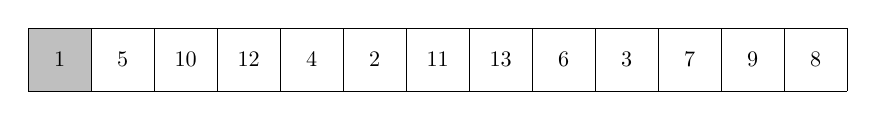
\begin{tikzpicture}[scale=0.8,transform shape]
                \draw (0,0) grid (13,1);
                \draw[fill=gray!50] (0,0)--(1,0)--(1,1)--(0,1)--cycle;
                \foreach \n/\x in {1/0,5/1,10/2,12/3,4/4,2/5,11/6,13/7,6/8,3/9,7/10,9/11,8/12}{
                    \node (\n) at (0.5+\x,0.5) {\n};

                }    
            \end{tikzpicture}
            \captionof{figure}{La partie triée est à gauche.}
        \end{center}

\end{frame}
\begin{frame}


        \begin{center}
            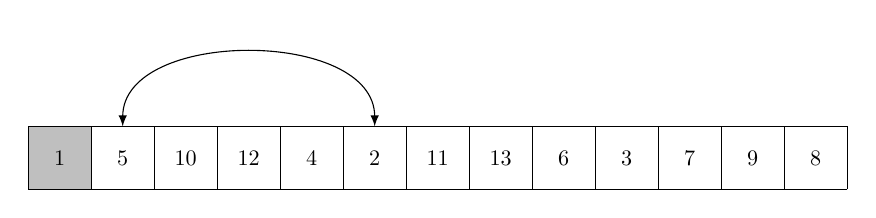
\begin{tikzpicture}[scale=0.8,transform shape]
                \draw (0,0) grid (13,1);
                \draw[fill=gray!50] (0,0)--(1,0)--(1,1)--(0,1)--cycle;
                \foreach \n/\x in {1/0,5/1,10/2,12/3,4/4,2/5,11/6,13/7,6/8,3/9,7/10,9/11,8/12}{
                    \node (\n) at (0.5+\x,0.5) {\n};

                }
    
                \draw[<->,>=latex] (1.5,1) to[bend left=90] (5.5,1);
    
            \end{tikzpicture}
            
            \captionof{figure}{Sélection du plus petit élément.}
        \end{center}
        \begin{center}
            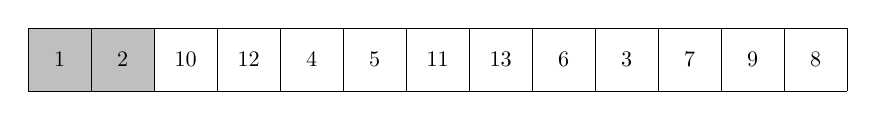
\begin{tikzpicture}[scale=0.8,transform shape]
                \draw[fill=gray!50] (0,0)--(2,0)--(2,1)--(0,1)--cycle;
                \draw (0,0) grid (13,1);
                \foreach \n/\x in {1/0,2/1,10/2,12/3,4/4,5/5,11/6,13/7,6/8,3/9,7/10,9/11,8/12}{
                    \node (\n) at (0.5+\x,0.5) {\n};

                }    
            \end{tikzpicture}
            \captionof{figure}{La partie triée est à gauche.}
        \end{center}

\end{frame}
\begin{frame}


    \begin{center}
        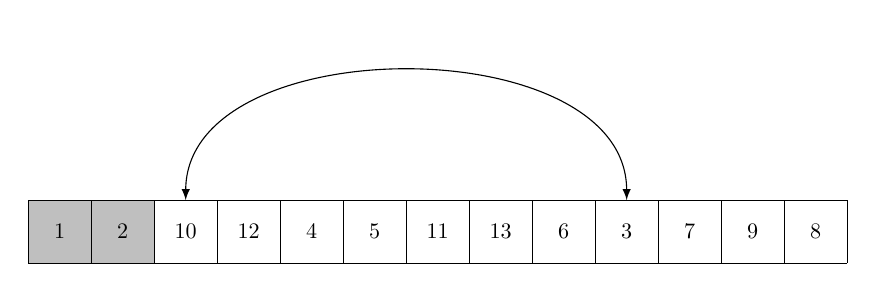
\begin{tikzpicture}[scale=0.8,transform shape]
            \draw[fill=gray!50] (0,0)--(2,0)--(2,1)--(0,1)--cycle;
            \draw (0,0) grid (13,1);

            \foreach \n/\x in {1/0,2/1,10/2,12/3,4/4,5/5,11/6,13/7,6/8,3/9,7/10,9/11,8/12}{
                \node (\n) at (0.5+\x,0.5) {\n};

            }

            \draw[<->,>=latex] (2.5,1) to[bend left=90] (9.5,1);

        \end{tikzpicture}
        
        \captionof{figure}{Sélection du plus petit élément.}
    \end{center}
    \begin{center}
        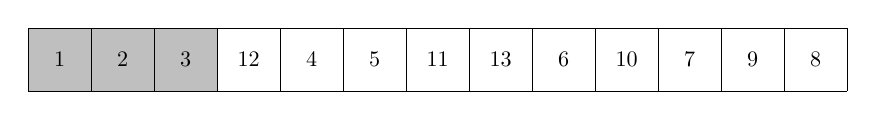
\begin{tikzpicture}[scale=0.8,transform shape]
            \draw[fill=gray!50] (0,0)--(3,0)--(3,1)--(0,1)--cycle;
            \draw (0,0) grid (13,1);
            \foreach \n/\x in {1/0,2/1,3/2,12/3,4/4,5/5,11/6,13/7,6/8,10/9,7/10,9/11,8/12}{
                \node (\n) at (0.5+\x,0.5) {\n};

            }    
        \end{tikzpicture}
        \captionof{figure}{La partie triée est à gauche.}
    \end{center}

\end{frame}
\subsection{Tri par insertion}
\begin{frame}
    \frametitle{Tri par insertion}

    \begin{itemize}
        \item Pour chaque carte du tas:
              \begin{itemize}
                  \item Tant que la carte précédente est plus petite
                  \item Échanger cette carte avec la carte en cours.
              \end{itemize}

    \end{itemize}

\end{frame}
\begin{frame}

    \begin{center}
        \centering
        \includegraphics[width=10cm]{ressources/jeu-coeur-melange.png}
        \end{center}
        \begin{center}
            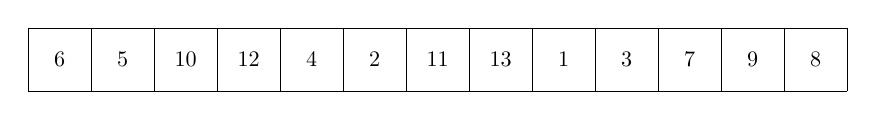
\begin{tikzpicture}[scale=0.8,transform shape]
                \draw (0,0) grid (13,1);
                \foreach \n/\x in {6/0,5/1,10/2,12/3,4/4,2/5,11/6,13/7,1/8,3/9,7/10,9/11,8/12}{
                    \node (\n) at (0.5+\x,0.5) {\n};

                }    
            \end{tikzpicture}
            \captionof{figure}{Modélisation}
        \end{center}

\end{frame}
\begin{frame}


        \begin{center}
            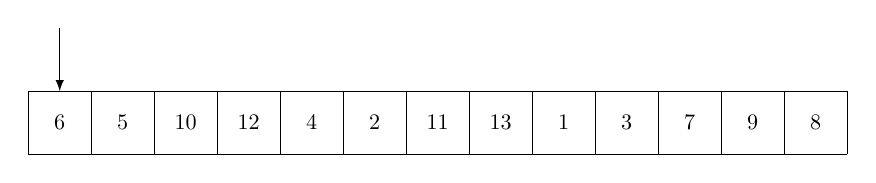
\begin{tikzpicture}[scale=0.8,transform shape]
                \draw (0,0) grid (13,1);
                \foreach \n/\x in {6/0,5/1,10/2,12/3,4/4,2/5,11/6,13/7,1/8,3/9,7/10,9/11,8/12}{
                    \node (\n) at (0.5+\x,0.5) {\n};

                }
    
                \draw[->,>=latex] (0.5,2) -- (0.5,1);
    
            \end{tikzpicture}
            
            \captionof{figure}{Carte en cours}
        \end{center}
        \begin{center}
            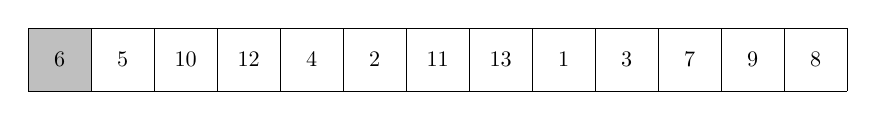
\begin{tikzpicture}[scale=0.8,transform shape]
                \draw[fill=gray!50] (0,0)--(1,0)--(1,1)--(0,1)--cycle;
                \draw (0,0) grid (13,1);
                
                \foreach \n/\x in {6/0,5/1,10/2,12/3,4/4,2/5,11/6,13/7,1/8,3/9,7/10,9/11,8/12}{
                    \node (\n) at (0.5+\x,0.5) {\n};

                }    
            \end{tikzpicture}
            \captionof{figure}{La partie triée est à gauche.}
        \end{center}

\end{frame}
\begin{frame}


    \begin{center}
        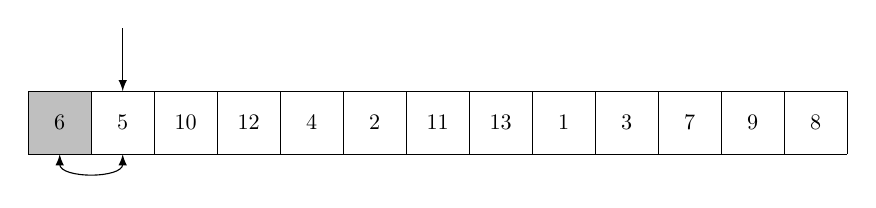
\begin{tikzpicture}[scale=0.8,transform shape]
            \draw[fill=gray!50] (0,0)--(1,0)--(1,1)--(0,1)--cycle;
            \draw (0,0) grid (13,1);
            \foreach \n/\x in {6/0,5/1,10/2,12/3,4/4,2/5,11/6,13/7,1/8,3/9,7/10,9/11,8/12}{
                \node (\n) at (0.5+\x,0.5) {\n};

            }

            \draw[->,>=latex] (1.5,2) -- (1.5,1);
            \draw[<->,>=latex] (0.5,0) to[bend right=90] (1.5,0);
        \end{tikzpicture}
        
        \captionof{figure}{Carte en cours}
    \end{center}
    \begin{center}
        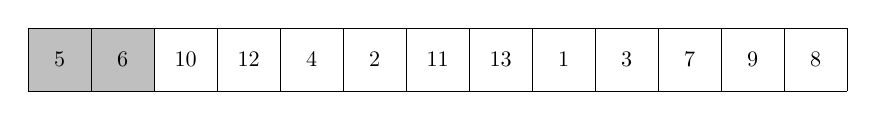
\begin{tikzpicture}[scale=0.8,transform shape]
            \draw[fill=gray!50] (0,0)--(2,0)--(2,1)--(0,1)--cycle;
            \draw (0,0) grid (13,1);
            
            \foreach \n/\x in {5/0,6/1,10/2,12/3,4/4,2/5,11/6,13/7,1/8,3/9,7/10,9/11,8/12}{
                \node (\n) at (0.5+\x,0.5) {\n};

            }    
        \end{tikzpicture}
        \captionof{figure}{La partie triée est à gauche.}
    \end{center}

\end{frame}
\section{Implémentation}
\subsection{Rappel: Passer un tableau à une fonction}
\subsection{Implémentations des tris}
\section{Études des implémentations}
\subsection{Terminaison}
\subsection{Correction}
\subsection{Complexité}
\end{document}